\documentclass{article}
\usepackage[utf8]{inputenc}
\usepackage[hmargin=2.5cm,vmargin=3cm,bindingoffset=0.5cm]{geometry}
\usepackage{graphicx}
\graphicspath{ {figures/} }
\usepackage{listings}
\usepackage{hyperref}
\usepackage{amsmath}
\usepackage{amssymb}
\usepackage{xcolor}
\usepackage{tcolorbox}
\usepackage{enumitem}
\usepackage{fancyhdr}
\renewcommand{\lstlistingname}{Auflistung}

% Define colors
\definecolor{thd-blue}{RGB}{0,82,147}
\definecolor{code-bg}{RGB}{245,245,245}
\definecolor{warning-bg}{RGB}{255,243,205}
\definecolor{info-bg}{RGB}{217,237,247}

% Configure listings
\lstset{
    backgroundcolor=\color{code-bg},
    basicstyle=\ttfamily\footnotesize,
    breakatwhitespace=false,
    breaklines=true,
    captionpos=b,
    commentstyle=\color{gray},
    frame=single,
    frameround=tttt,
    framesep=5pt,
    numbers=left,
    numbersep=5pt,
    numberstyle=\tiny\color{gray},
    rulecolor=\color{black},
    showspaces=false,
    showstringspaces=false,
    showtabs=false,
    stepnumber=1,
    stringstyle=\color{thd-blue},
    tabsize=2,
    title=\lstname
}

% Configure tcolorbox
\tcbuselibrary{skins,breakable}

% Define custom boxes
\newtcolorbox{infobox}{
    colback=info-bg,
    colframe=thd-blue,
    arc=3mm,
    breakable,
    left=5mm,
    right=5mm,
    top=3mm,
    bottom=3mm
}

\newtcolorbox{warningbox}{
    colback=warning-bg,
    colframe=orange,
    arc=3mm,
    breakable,
    left=5mm,
    right=5mm,
    top=3mm,
    bottom=3mm
}

% Configure headers and footers
\pagestyle{fancy}
\fancyhf{}
\fancyhead[L]{\textcolor{thd-blue}{\textbf{CurveBall CTF Challenge}}}
\fancyhead[R]{\textcolor{thd-blue}{\thepage}}
\fancyfoot[C]{\textcolor{gray}{\small Kryptologie 2 - TH Deggendorf}}
\renewcommand{\headrulewidth}{0.5pt}
\renewcommand{\headrule}{\hbox to\headwidth{\color{thd-blue}\leaders\hrule height \headrulewidth\hfill}}

\begin{document}

\pagenumbering{alph}
\begin{titlepage}
  \begin{center}
    
\includegraphics[width=\textwidth]{THD-Logo.pdf}
    \vspace{1cm}
    \rule{1\textwidth}{1mm} \\[0.3cm]
    \textsc{\scshape \huge Bachelor Cyber Security}\\
    \rule{1\textwidth}{1mm} \\[2cm]
    {
      \vspace{1cm}
      \Large \textbf{Kryptologie 2}
      \vspace{3cm}
      \Large \textbf{Projektbericht}
    }\\[0.5cm]
    \LARGE \textbf{Ausarbeitung Cryptochallenge: CurveBall}\\[2cm]
    \begin{minipage}[t]{0.4\textwidth}
      \begin{flushleft}
        \normalsize \emph{Autor:}\\[0.3cm]
        Manuel Friedl, Matrikel-Nr.: 1236626\\
        Christof Renner, Matrikel-Nr.: 22301943
      \end{flushleft}
    \end{minipage}
    \begin{minipage}[t]{0.5\textwidth}
      \begin{flushright}
        \normalsize \emph{Betreuer:}\\[0.3cm]
        Prof. Dr. Martin Schramm
      \end{flushright}
    \end{minipage}\\[3cm]
    {\large Deggendorf – 28.07.2025\\}
  \end{center}
\end{titlepage}

\newpage
\pagenumbering{Roman}
\thispagestyle{empty}

\newpage
\tableofcontents
\thispagestyle{empty}
\newpage

\pagenumbering{arabic}
\setcounter{page}{1}

\section{Einführung}

\begin{infobox}
\textbf{Willkommen zur CurveBall CTF Challenge!}

Diese Challenge behandelt eine der kritischsten Sicherheitslücken in der Windows-Geschichte: CVE-2020-0601, bekannt als \textit{CurveBall}. Sie lernen die Grundlagen der Elliptic Curve Cryptography (ECC) kennen und verstehen, wie Schwachstellen in kryptographischen Implementierungen ausgenutzt werden können.
\end{infobox}

\vspace{0.5cm}

\section{Systemvoraussetzungen}

\begin{itemize}[leftmargin=1.5cm]
    \item \textbf{Docker} und \textbf{Docker Compose} (Version 20.10 oder höher)
    \item \textbf{Webbrowser} (empfohlen: Firefox oder Chrome)
    \item \textbf{Grundlegende Kenntnisse:}
    \begin{itemize}
        \item Kryptographie-Grundlagen
        \item Python-Programmierung
        \item Umgang mit Zertifikaten
    \end{itemize}
    \item \textbf{Texteditor oder IDE} für die Bearbeitung von Code
    \item \textbf{Mindestens 2 GB freier Arbeitsspeicher}
\end{itemize}

\section{Challenge-Setup und Start}

\begin{warningbox}
\textbf{Wichtiger Hinweis:} Stellen Sie sicher, dass Docker auf Ihrem System installiert und gestartet ist, bevor Sie mit dem Setup beginnen.
\end{warningbox}

\begin{enumerate}[leftmargin=1.5cm]
    \item \textbf{Repository klonen:}
    \begin{lstlisting}[language=bash]
git clone https://mygit.th-deg.de/cr02943/kryptologie2-curveball
    \end{lstlisting}

    \item \textbf{Zum Challenge-Verzeichnis navigieren:}
    \begin{lstlisting}[language=bash]
cd kryptologie2-curveball/curveball-ctf/
    \end{lstlisting}
    
    \item \textbf{Challenge-Umgebung starten:}
    \begin{lstlisting}[language=bash]
docker-compose up --build -d
    \end{lstlisting}
    
    \item \textbf{Challenge aufrufen:}
    
    Öffnen Sie Ihren Webbrowser und navigieren Sie zu:
    \begin{center}
        \textcolor{thd-blue}{\textbf{\large https://localhost:8443}}
    \end{center}
\end{enumerate}

\begin{infobox}
\textbf{Zertifikatswarnung:} Da die Challenge ein selbstsigniertes Zertifikat verwendet, erhalten Sie eine Sicherheitswarnung im Browser. Akzeptieren Sie das Zertifikat, um fortzufahren.
\end{infobox}

\begin{figure}[htbp]
  \centering
  \fbox{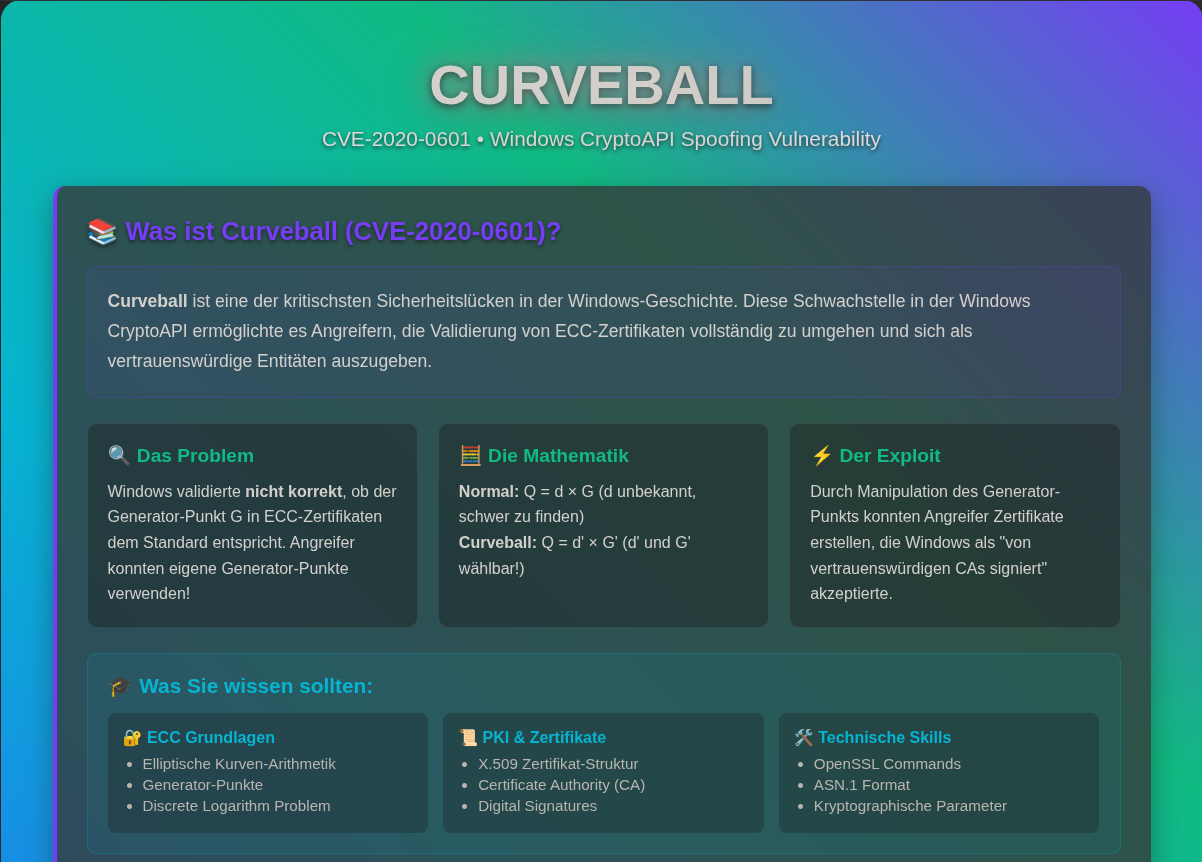
\includegraphics[width=0.9\textwidth]{Page.png}}
  \caption{\textcolor{thd-blue}{\textbf{Challenge Weboberfläche - Hauptseite}}}
  \label{fig:webpage}
\end{figure}

\clearpage

\section{Challenge-Struktur}

Die CurveBall CTF-Challenge ist modular aufgebaut und besteht aus vier aufeinander aufbauenden Bereichen. Jeder Bereich behandelt spezifische Aspekte der ECC-Kryptographie und der CurveBall-Schwachstelle.

\vspace{0.5cm}

\subsection{Einführungsbereich}

\begin{infobox}
\textbf{Theoretische Grundlagen}

Der Einführungsbereich vermittelt das notwendige Hintergrundwissen für die praktischen Challenges.
\end{infobox}

\textbf{Inhalte:}
\begin{itemize}[leftmargin=1.5cm]
    \item \textbf{Elliptic Curve Cryptography (ECC):} Mathematische Grundlagen und Algorithmen
    \item \textbf{CVE-2020-0601 Schwachstelle:} Technische Details und Auswirkungen
    \item \textbf{Historischer Kontext:} Entdeckung durch die NSA und globale Auswirkungen
    \item \textbf{Kryptographische Konzepte:} Schlüsselgenerierung, Signaturen und Zertifikate
\end{itemize}

\vspace{0.8cm}

\subsection{Challenge 1: ECC-Grundlagen}

\begin{tcolorbox}[colback=thd-blue!10,colframe=thd-blue,title=\textbf{Lernziele}]
\begin{itemize}[leftmargin=1cm]
    \item Verstehen der mathematischen Struktur elliptischer Kurven
    \item Praktische Anwendung von Punktoperationen auf elliptischen Kurven
    \item Implementierung und Verständnis von ECC-Algorithmen
\end{itemize}
\end{tcolorbox}

\textbf{Praktische Aufgaben:}
\begin{itemize}[leftmargin=1.5cm]
    \item Berechnung von Punktaddition und -multiplikation auf elliptischen Kurven
    \item Analyse und Manipulation der Parameter einer elliptischen Kurve
    \item Implementierung grundlegender ECC-Operationen in JavaScript
\end{itemize}

\vspace{0.8cm}

\newpage

\subsection{Challenge 2: Zertifikatsgenerierung}

\begin{tcolorbox}[colback=thd-blue!10,colframe=thd-blue,title=\textbf{Lernziele}]
\begin{itemize}[leftmargin=1cm]
    \item Verstehen der Struktur und des Formats von X.509-Zertifikaten
    \item Erstellung und Verarbeitung von Certificate Signing Requests (CSR)
    \item Manipulation und Analyse von Zertifikatsparametern
\end{itemize}
\end{tcolorbox}

\textbf{Praktische Aufgaben:}
\begin{itemize}[leftmargin=1.5cm]
    \item Generierung von ECC-Schlüsselpaaren für verschiedene Kurven
    \item Erstellung, Signierung und Validierung von X.509-Zertifikaten
    \item Forensische Analyse von Zertifikatsstrukturen und -inhalten
\end{itemize}

\vspace{0.8cm}

\subsection{Challenge 3: Kurvenmanipulation}

\begin{tcolorbox}[colback=orange!10,colframe=orange,title=\textbf{Lernziele}]
\begin{itemize}[leftmargin=1cm]
    \item Verstehen der technischen Details der CurveBall-Schwachstelle
    \item Praktische Manipulation von elliptischen Kurvenparametern
    \item Ausnutzung von Schwächen in der Zertifikatsvalidierung
\end{itemize}
\end{tcolorbox}

\textbf{Praktische Aufgaben:}
\begin{itemize}[leftmargin=1.5cm]
    \item Modifikation von elliptischen Kurvenparametern (a, b, p)
    \item Erstellung von Zertifikaten mit manipulierten Kurven
    \item Demonstration der Umgehung der Windows CryptoAPI-Validierung
\end{itemize}

\vspace{0.8cm}

\subsection{Challenge 4: Signature-Spoofing}

\begin{tcolorbox}[colback=red!10,colframe=red,title=\textbf{Lernziele}]
\begin{itemize}[leftmargin=1cm]
    \item Praktische Ausnutzung der CVE-2020-0601 Schwachstelle
    \item Erstellung und Validierung gefälschter digitaler Signaturen
    \item Verstehen der weitreichenden Auswirkungen auf PKI-Systeme
\end{itemize}
\end{tcolorbox}

\textbf{Praktische Aufgaben:}
\begin{itemize}[leftmargin=1.5cm]
    \item Implementierung von erweiterten Signature-Spoofing-Techniken
    \item Validierung und Verifikation manipulierter Zertifikatsketten
    \item Umfassende Demonstration der Sicherheitslücke und ihrer Auswirkungen
\end{itemize}

\clearpage

\section{Container-Management und Troubleshooting}

\subsection{Grundlegende Docker-Befehle}

\begin{warningbox}
\textbf{Wichtig:} Führen Sie alle Befehle im Verzeichnis \texttt{curveball-ctf/} aus.
\end{warningbox}

\subsubsection{Challenge stoppen}
\begin{lstlisting}[language=bash]
docker-compose down
\end{lstlisting}

\subsubsection{Container neu starten}
\begin{lstlisting}[language=bash]
docker-compose restart
\end{lstlisting}

\subsubsection{Logs anzeigen}
\begin{lstlisting}[language=bash]
# Alle Logs anzeigen
docker-compose logs -f

# Nur Webserver-Logs anzeigen
docker-compose logs -f webserver
\end{lstlisting}

\subsubsection{Container-Status überprüfen}
\begin{lstlisting}[language=bash]
docker-compose ps
\end{lstlisting}

\subsubsection{Komplette Neuinstallation}
\begin{lstlisting}[language=bash]
# Container stoppen und entfernen
docker-compose down --volumes --remove-orphans

# Images neu erstellen und starten
docker-compose up --build -d
\end{lstlisting}

\vspace{0.8cm}

\end{document}